\chapter{Courant Continu} \label{subsec:dc_circuit_theory}
La théorie des circuits en courant continu (DC) pose les bases de l’électronique en
décrivant le comportement des tensions et courants statiques (invariants dans le temps)
dans des boucles fermées.\\

\begin{figure}[!h]
  \centering
  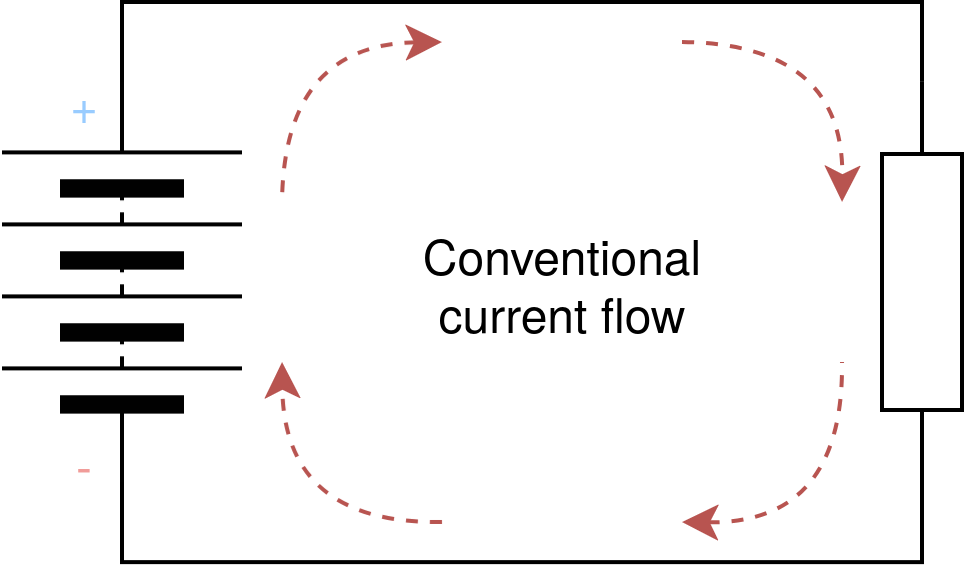
\includegraphics[width=0.6\textwidth]{current-flow.png}
  \caption{Le flux conventionnel du courant, de \(+\) vers --}
\end{figure}

\section{Les unités traitées} \label{subsec:units}
Avant d’aborder les circuits et les composants, il est important de définir
les \textit{unités fondamentales} qui constituent le langage de l’électronique.
À la base se trouve la \textbf{charge électrique}, la grandeur fondamentale
qui sous-tend toutes les interactions électriques. De la charge découle le \textbf{courant
électrique}, le flux de charges à travers un conducteur, et la \textbf{tension},
la différence de potentiel qui provoque ce flux. Les matériaux s’opposent au
mouvement des charges via leur \textbf{résistance}, tandis que les notions
d’\textbf{énergie} et de \textbf{puissance} permettent de décrire comment les circuits
stockent et délivrent un travail utile. Ensemble, ces unités établissent le
cadre à travers lequel nous mesurons et analysons les phénomènes électriques.\par
\vspace{\baselineskip}
\subsection{Charge électrique}\label{subsec:electric_charge}
La charge électrique est une propriété fondamentale de la matière ; elle permet
les interactions via les champs électromagnétiques. Elle se quantifie en \textbf{coulombs
(\unit{\coulomb})}. Il existe deux types de charges électriques, qualifiées de
positive et négative. Les charges de même signe se repoussent, tandis que les charges
de signes opposés s’attirent. Dans la matière ordinaire, le total des charges
positives et négatives est équilibré, une condition appelée neutralité électrique.
Les électrons (--) et les protons (\(+\)) sont les principaux porteurs de charge électrique.

\begin{figure}[H]
  \centering
  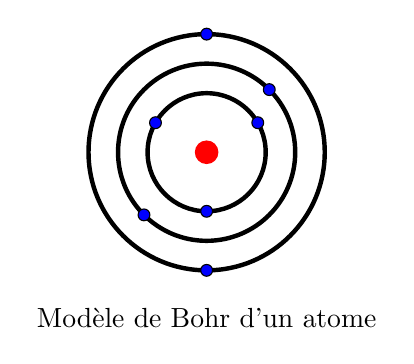
\begin{tikzpicture}[scale=0.75]
    \fill[red] (0,0) circle (0.2);
    \draw[ultra thick] (0,0) circle (1);
    \draw[ultra thick] (0,0) circle (1.5);
    \draw[ultra thick] (0,0) circle (2);
    \foreach \theta in {30, 150, 270}
    \draw[fill=blue] (\theta:1) circle (0.1);

    \foreach \theta in {45, 225}
    \draw[fill=blue] (\theta:1.5) circle (0.1);

    \foreach \theta in {90, 270}
    \draw[fill=blue] (\theta:2) circle (0.1);
    \node[below=1em] at (0, -2) {Modèle de Bohr d'un atome};
  \end{tikzpicture}
\end{figure}

Dans les contextes industriels et d’ingénierie, l’ampère-heure (Ah) --et ses
sous-multiples-- est couramment utilisé à la place du coulomb, notamment pour
indiquer la capacité d’une batterie, auquel cas :
\[
  1~\unit{\ampere\hour} = 3\,600~\unit{\coulomb}.
\]
Cette unité permet d’estimer facilement combien de temps une batterie peut
fournir un courant donné :
\begin{example}:\newline
Une batterie de 30\unit{\ampere\hour}
délivrant 1\unit{\ampere} durerait théoriquement 30\unit{\hour} (ou 15\unit{\hour} à
2\unit{\ampere}), et ainsi de suite.
\end{example}
\begin{Note}
\textbf{Points clés de la charge électrique (loi de Coulomb) :}
\begin{enumerate}
  \item Il existe deux types de charge : positive et négative.
  \item Les charges de même type se repoussent mutuellement.
  \item Les charges de types opposés s’attirent mutuellement.
\end{enumerate}
\end{Note}

\subsection{Intensité du courant} \label{subsec:current}

\begin{Note}
	La notion de courant alternatif sera abordée dans la section (Work In Progress) \Cref{subsec:ac_circuit_theory}.
\end{Note}

Un courant électrique est le mouvement collectif des porteurs de charge —
typiquement des électrons — à travers un milieu conducteur, entraîné par
la force électromagnétique.
Un courant de 1 ampère correspond au passage d’une charge de \textbf{1 coulomb}
par seconde à travers une section de conducteur :
\[
  I = \frac{Q}{t}
\]
où :
\begin{itemize}
  \item \(I\) est le courant électrique (en ampères),
  \item \(Q\) est la charge (en coulombs),
  \item \(t\) est le temps (en secondes).
\end{itemize}

\begin{figure}[H]
    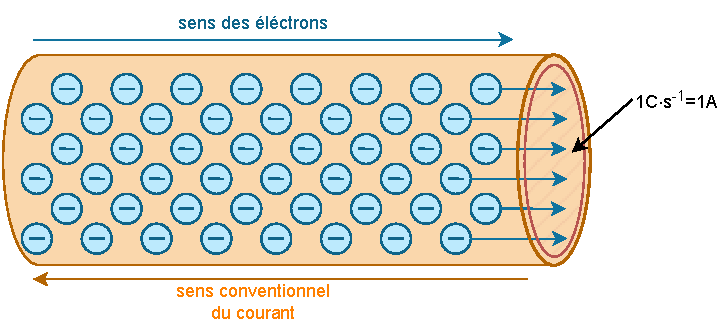
\includegraphics[width=0.7\textwidth]{electron-flow.pdf}
    \caption{Flux de courant dans un conducteur}
\end{figure}
\begin{Todo}
	Aborder la notion de densité de courant. Peut-\^etre dans une section li\'ee \`a l'\'electromagn\'etisme.
	\[
	\vec{j}_S=\int_0^e\vec{j}_S\cdot\vec{dl}
	\]
\end{Todo}

\begin{Note}
\vspace{\baselineskip}
\textbf{Points clés de l’intensité :}
\begin{enumerate}
  \item Elle traduit la vitesse de déplacement des charges dans un conducteur.
  \item Elle est directement liée à la charge et au temps (\(I = Q/t\)).
  \item Elle constitue, avec la tension, la base du calcul de la puissance électrique (\(P = U \cdot I\)).
\end{enumerate}
\end{Note}

\subsection{La tension électrique}
\begin{Note}
	La notion de courant alternatif sera abordée dans la section (Work In Progress) \Cref{subsec:ac_circuit_theory}.
\end{Note}

La \textbf{tension électrique} (ou différence de potentiel) est la cause
qui met en mouvement les charges électriques dans un circuit. Elle
correspond au travail nécessaire pour déplacer une charge électrique
unitaire entre deux points. Elle se mesure en \textbf{volts
(\unit{\volt})}.

Mathématiquement, la tension est définie comme :
\[
  U = \frac{W}{Q}
\]
où \(U\) est la tension en volts, \(W\) le travail en joules, et \(Q\) la charge
en coulombs. Ainsi, un volt équivaut à un joule par coulomb :
\[
1V=1\frac{J}{C}
\]

% \begin{figure}[!h]
%   \centering
%   \conditionalincludegraphics{src/assets/voltage}{true}{0.5}
%   \caption{Représentation d’une différence de potentiel entre deux points}
% \end{figure}

\vspace{\baselineskip}
\begin{Note}
\textbf{Points clés de la tension :}
\begin{enumerate}
  \item Elle est mesurée entre deux points (différence de potentiel).
  \item Elle constitue la “force motrice” des circuits électriques.
  \item Son unité est le volt, équivalent à un joule par coulomb.
\end{enumerate}
\end{Note}


\section{Composants de base} \label{subsec:basic_components}
\subsection{Résistances} \label{subsec:resistors}
Une résistance est un composant passif qui limite l’intensité du courant
et transforme une partie de l’énergie électrique en chaleur.
Sa relation fondamentale est donnée par la loi d’Ohm :
\[
U = R \cdot I
\]
où \(R\) est exprimée en ohms (\unit{\ohm}).

\begin{figure}[H]
    \centering
    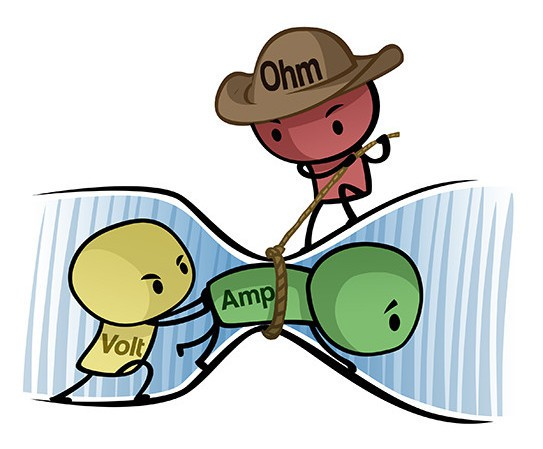
\includegraphics[width=0.6\textwidth]{ohms-law-cartoon}
    \caption{
        \centering
        R\'esistance \'electrique expliqu\'ee par un cowboy.\\
        \textbf{Source~:}
        \href{https://build-electronic-circuits.com/ohms-law}{build-electronic-circuits.com}
    }

\end{figure}


\textbf{Rôle principal :} les résistances servent à fixer des tensions, limiter
le courant dans des composants sensibles (par exemple une LED), ou réaliser
des ponts diviseurs de tension \Cref{fig:voltage-divider}. Elles existent en version fixe (valeur constante)
ou variable (potentiomètres, rhéostats).

Leur valeur est souvent indiquée par un code de couleurs :

\begin{table}[H]
\centering
\caption{Code des couleurs pour les résistances (4 bandes)}
\label{tab:resistor_colors}
\begin{tabular}{|l|c|c|c|r|}
\hline
\textbf{Couleur} & \textbf{Chiffre} & \textbf{Multiplicateur} & \textbf{Tolérance} & \textbf{Exemple} \\
\hline

\begin{tikzpicture}\fill[black] (0,0) rectangle (0.4,0.4); \end{tikzpicture} Noir & 0 & $10^0$ & - & \si{10\ohm} \\

\begin{tikzpicture}\fill[brown] (0,0) rectangle (0.4,0.4); \end{tikzpicture} Marron & 1 & $10^1$ & ±1\% & \si{10\ohm} \\

\begin{tikzpicture}\fill[red] (0,0) rectangle (0.4,0.4); \end{tikzpicture} Rouge & 2 & $10^2$ & ±2\% & \si{200\ohm} \\

\begin{tikzpicture}\fill[orange] (0,0) rectangle (0.4,0.4); \end{tikzpicture} Orange & 3 & $10^3$ & - & \si{3e3\ohm} \\

\begin{tikzpicture}\fill[yellow] (0,0) rectangle (0.4,0.4); \end{tikzpicture} Jaune & 4 & $10^4$ & - & \si{40e3\ohm} \\

\begin{tikzpicture}\fill[green] (0,0) rectangle (0.4,0.4); \end{tikzpicture} Vert & 5 & $10^5$ & ±0.5\% & \si{500e3\ohm} \\

\begin{tikzpicture}\fill[blue] (0,0) rectangle (0.4,0.4); \end{tikzpicture} Bleu & 6 & $10^6$ & ±0.25\% & \si{1e6\ohm} \\

\begin{tikzpicture}\fill[violet] (0,0) rectangle (0.4,0.4); \end{tikzpicture} Violet & 7 & $10^7$ & ±0.1\% & \si{10e6\ohm} \\

\begin{tikzpicture}\fill[gray] (0,0) rectangle (0.4,0.4); \end{tikzpicture} Gris & 8 & $10^8$ & ±0.05\% & \si{100e6\ohm} \\
\begin{tikzpicture}\fill[white] (0,0) rectangle (0.4,0.4); \draw (0,0) rectangle (0.4,0.4); \end{tikzpicture} Blanc & 9 & $10^9$ & - & \si{1e9\ohm} \\
\begin{tikzpicture}\fill[gold] (0,0) rectangle (0.4,0.4); \end{tikzpicture} Or & - & $10^{-1}$ & ±5\% & \si{0.1\ohm} \\
\begin{tikzpicture}\fill[silver] (0,0) rectangle (0.4,0.4); \end{tikzpicture} Argent & - & $10^{-2}$ & ±10\% & \si{0.01\ohm} \\
\hline
\end{tabular}
\end{table}

\textbf{Association en série :}
\begin{figure}[H]
    \centering
    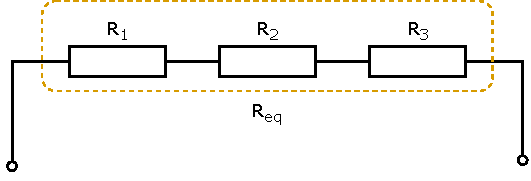
\includegraphics[width=0.8\textwidth]{resistor-series.pdf}
    \caption{\centering
    Association en série de résistances.\\
    La résistance équivalente est la somme des résistances individuelles~:\\
    \(R_{eq} = R_1 + R_2\).}
\end{figure}

\textbf{Association en parallèle :}
\begin{figure}[H]
    \fcapside[\FBwidth]{%
        \caption[R\'esistances en parall\`ele.]{
        Association en parallèle de résistances.\\
        L’inverse de la résistance équivalente est la somme des inverses des résistances individuelles~:
        \vspace{1ex}

        \(\dfrac{1}{R_{eq}} = \dfrac{1}{R_1} + \dfrac{1}{R_2}\).
        }%
        \label{fig:resistor-parallel}%
    }{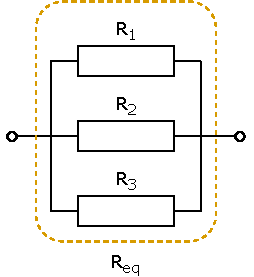
\includegraphics[width=0.4\textwidth]{resistor-parallel.pdf}}%
\end{figure}

\textbf{Pont diviseur de tension :}
\begin{figure}[H]
    \fcapside[\FBwidth]{%
        \caption[Pont diviseur de tension.]{
        Pont diviseur de tension.\\La tension de sortie \(V_{out}\) est une
        fraction de la tension d’entrée \(V_{in}\), déterminée par les valeurs
        des résistances \(R_1\) et \(R_2\)~:
        \vspace{1ex}

        \(V_{out} = V_{in}\cdot\dfrac{R_2}{R_1 + R_2}\)
        }%
        \label{fig:voltage-divider}%
    }{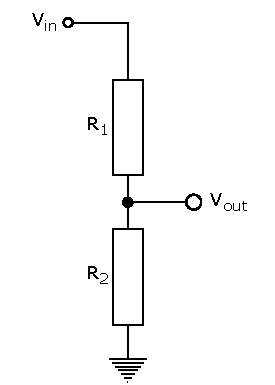
\includegraphics[width=0.4\textwidth]{voltage-divider.pdf}}%
\end{figure}


\textbf{Effet Joule :} lorsqu’un courant traverse une résistance, l’énergie
électrique est dissipée sous forme de chaleur. La puissance thermique dégagée
est donnée par :
\[
P = U \cdot I = R \cdot I^2 = \frac{U^2}{R}.
\]
Cet échauffement, appelé \emph{effet Joule}, peut être utile (ex. : radiateurs,
fils chauffants) ou problématique (surchauffe des composants, pertes énergétiques).
Les résistances sont donc conçues avec une puissance nominale (en watts, \unit{\watt})
qu’il ne faut pas dépasser pour éviter leur destruction.

En pratique, les résistances existent sous différentes formes :
à couche carbone, à film métallique, bobinées ou intégrées dans des circuits imprimés.
Leur choix dépend à la fois de leur valeur, de leur tolérance et de leur puissance maximale.

\subsection{Condensateurs} \label{subsec:capacitors}
Un condensateur stocke de l’énergie dans un champ électrique
entre deux armatures séparées par un isolant (le diélectrique).
Sa relation fondamentale est :
\[
Q = C \cdot U
\]
où \(C\) est la capacité en farads (\unit{\farad}).
Les condensateurs laissent passer les signaux variables (AC)
et bloquent les signaux constants (DC).
Ils sont utilisés pour filtrer les alimentations,
réaliser des circuits résonants, ou encore découpler des étages électroniques.

Les types de condensateurs courants incluent :
\begin{itemize}
  \item \textbf{Condensateurs céramiques :} petit format, faible ESR (r\'esistance \'equivalente en s\'erie), haute fréquence.
        Utilisés pour découplage, filtrage HF et circuits résonants.
  \item \textbf{Condensateurs électrolytiques :} grande capacité, polarité à respecter,
        adaptés au filtrage d’alimentation et au stockage d’énergie.
  \item \textbf{Condensateurs à film :} faible perte, non polarisés, haute stabilité.
        Applications : circuits audio, filtres, temporisations.
  \item \textbf{Condensateurs tantale :} compacts et stables, polarité à respecter,
        utilisés pour alimentation stable et découplage.
  \item \textbf{Supercondensateurs / ultracapacitors :} très grande capacité, décharge rapide,
        pour sauvegarde d’énergie ou alimentation tampon.
  \item \textbf{Condensateurs à mica :} grande précision, faible perte, haute fréquence.
        Utilisés pour oscillateurs HF et circuits radio.
  \item \textbf{Condensateurs variables :} capacité réglable mécaniquement ou électroniquement,
        pour syntonisation\footnote{Glossaire~: \gls{syntonisation}}  d’oscillateurs ou ajustement de filtres.
\end{itemize}
\begin{Note}
	Les notions de filtrage, fr\'equences et impédances seront abordées dans la section (Work In Progress) \Cref{subsec:ac_circuit_theory}.
\end{Note}

\textbf{Association en série :}
\begin{figure}[H]
    \centering
    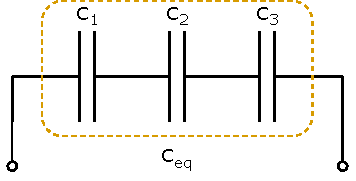
\includegraphics[width=0.6\textwidth]{capacitor-series.pdf}
    \caption{\centering
    Association en série de condensateurs.\\
    L’inverse de la capacité équivalente est la somme des inverses des capacités individuelles
    ~:\\
    \(\dfrac{1}{C_{eq}} = \dfrac{1}{C_1} + \dfrac{1}{C_2}\)}
\end{figure}

\textbf{Association en parallèle :}
\begin{figure}[H]
    \fcapside[\FBwidth]{%
        \caption[Condensateurs en parall\`ele.]{
        Association en parallèle de condensateurs.\\
        La capacité équivalente est la somme des capacités individuelles~:\\
        \(C_{eq} = C_1 + C_2\).}%
        \label{fig:capacitor-parallel}%
    }{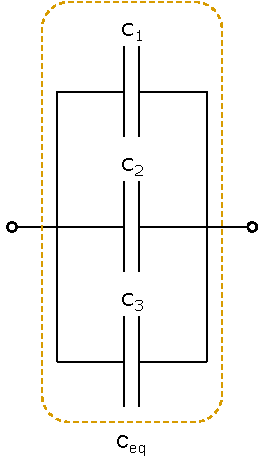
\includegraphics[width=0.4\textwidth]{capacitor-parallel.pdf}}%
\end{figure}

\subsection{Inductances} \label{subsec:inductors}
Une inductance (ou bobine) est un composant passif qui stocke de l’énergie
dans un champ magnétique lorsqu’un courant la traverse.
\[
u(t) = L \frac{di(t)}{dt}
\]
où \(L\) est l’inductance (en henrys, \unit{\henry}) et \(i(t)\) le courant instantané.

\vspace{\baselineskip}
Lorsque le courant est constant (\(\frac{di}{dt} = 0\)), la tension aux bornes
de l’inductance est nulle (\(u = 0\)). Autrement dit, une inductance se comporte
comme un \textbf{court-circuit idéal} en régime continu. L’inductance ne s’oppose
donc pas au courant constant, mais uniquement aux variations de courant et \'emet un champ
magnétique constant.


\subsection{Diodes} \label{subsec:diodes}
Une diode est un composant semi-conducteur qui laisse passer le courant
dans un sens (polarisation directe) et le bloque dans l’autre (polarisation inverse).
Sa caractéristique \(I(V)\) est non linéaire et se rapproche
d’un interrupteur dirigé.
\begin{figure}[H]
    \centering
    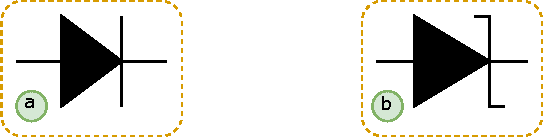
\includegraphics[width=0.5\textwidth]{diodes.pdf}
    \caption{\newline
        \textbf{a)} Symbole d’une diode.\\
        \textbf{b)} Symbole d’une diode Zener.
    }
\end{figure}
Les applications courantes impliquent le redressement dans les alimentations, la protection contre l’inversion de polarité
ou la régulation de tension (diodes Zener).
Certaines diodes spéciales, comme les LED, convertissent l’énergie électrique en lumière.

\subsection{Transistors} \label{subsec:transistors}
Le transistor est un composant actif central de l’électronique moderne.
Il peut amplifier un signal ou agir comme un interrupteur contrôlé.
On distingue principalement :
\begin{itemize}
  \item \textbf{BJT (bipolaire)} : le courant de base contrôle
  le courant de collecteur.
  \item \textbf{MOSFET (à effet de champ)} : la tension de grille contrôle
  le courant de drain.
\end{itemize}

\begin{figure}[H]
    \centering
    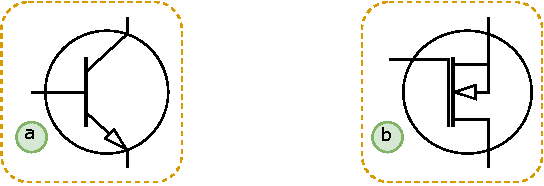
\includegraphics[width=0.6\textwidth]{transistors.pdf}
    \caption{\centering\newline
        \textbf{a)} Symbole d’un transistor NPN (BJT).\\
        \textbf{b)} Symbole d’un transistor N-channel (MOSFET).
    }
\end{figure}

Les transistors sont utilisés dans les amplificateurs,
les circuits logiques, les régulateurs, et constituent les briques de base des processeurs.
\section{Lois de Kirchhoff} \label{subsec:kirchhoff}
\subsection{Loi des nœuds} \label{subsec:noeuds}

\subsection{Loi des mailles} \label{subsec:mailles}

\section{Théorèmes de Norton et de Thévenin} \label{subsec:norton_thevenin}
